% Compile with: lualatex cardioid.tex
\documentclass[11pt]{article}

\usepackage{amsmath, amssymb}
\usepackage{tikz}
\usepackage[a4paper, margin=2.5cm]{geometry}
\usepackage[colorlinks=true, urlcolor=blue]{hyperref}
\usepackage{fancyhdr}

\pagestyle{fancy}
\fancyhf{}
\renewcommand{\headrulewidth}{0pt}
\fancyfoot[L]{\small Junzhe Wang ~\textperiodcentered~
  \href{mailto:junzhe.wang2002@gmail.com}{\texttt{junzhe.wang2002@gmail.com}}}
\fancyfoot[R]{\small Last edited: \today\ ~\textperiodcentered~ p.\,\thepage}

\title{The Cardioid}
\author{}
\date{}

\begin{document}

\maketitle
\thispagestyle{fancy}

\section{Definition}

A \emph{cardioid} (from the Greek \emph{kardia}, heart) is the plane curve
traced by a point fixed on the circumference of a circle that rolls, without
slipping, around a second circle of the same radius. It is therefore a special
case of an \emph{epicycloid}, the one with exactly one cusp.

\section{Parametric equations}

For a rolling radius $a$, the variant drawn in \emph{Learn Programming with
OCaml} (Program~3) is
\begin{equation}
  \begin{cases}
    x(\theta) = a\,(1 - \sin\theta)\,\cos\theta \\
    y(\theta) = a\,(1 - \sin\theta)\,\sin\theta
  \end{cases}
  \qquad \theta \in [0, 2\pi].
\end{equation}
Equivalently, in polar coordinates $(r, \theta)$ the curve is
\begin{equation}
  r(\theta) = a\,(1 - \sin\theta),
\end{equation}
which reads directly as: the distance from the origin swells to $2a$ at
$\theta = -\frac{\pi}{2}$ (the bottom of the heart) and collapses to $0$ at
$\theta = \frac{\pi}{2}$, producing the cusp.

\begin{center}
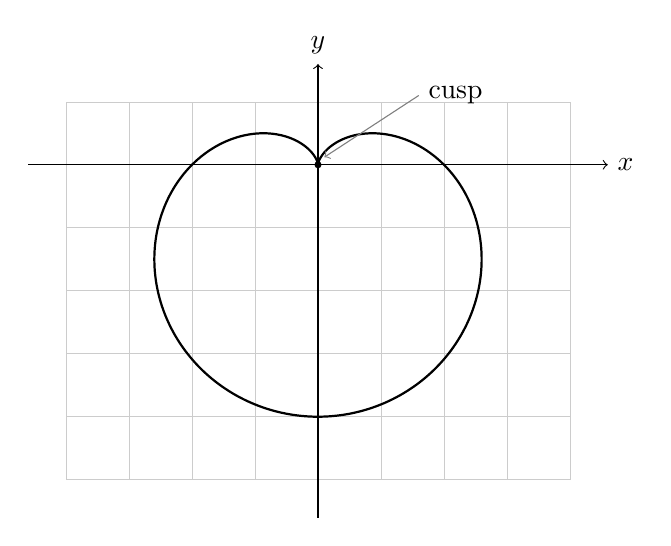
\begin{tikzpicture}[scale=1.6]
  \draw[very thin, gray!40] (-2, -2.5) grid[step=0.5] (2, 0.5);
  \draw[->] (-2.3, 0) -- (2.3, 0) node[right] {$x$};
  \draw[->] (0, -2.8) -- (0, 0.8) node[above] {$y$};
  \draw[thick, domain=0:360, samples=400, smooth]
    plot ({(1 - sin(\x)) * cos(\x)}, {(1 - sin(\x)) * sin(\x)});
  \fill (0, 0) circle (0.8pt);
  \draw[gray, ->] (0.8, 0.55) -- (0.05, 0.06);
  \node[right] at (0.8, 0.55) {cusp};
\end{tikzpicture}

\smallskip
The cardioid $r = 1 - \sin\theta$ (that is, $a = 1$).
\end{center}

\section{Properties}

For the cardioid of parameter $a$:
\begin{itemize}
  \item \textbf{Cusp.} At $\theta = \frac{\pi}{2}$ the factor $1 - \sin\theta$
    vanishes, so the point reaches the origin with zero speed and reverses
    smoothly: the single sharp point characteristic of the curve.
  \item \textbf{Area.} The enclosed area is
    $\displaystyle \frac{1}{2}\int_0^{2\pi} r(\theta)^2 \,\mathrm{d}\theta
      = \frac{3}{2}\pi a^2$
    --- exactly six times the area of the rolling circle of radius $a/2$\,%
    \footnote{With the rolling-circle construction, a cardioid of polar
    parameter $a$ is generated by circles of radius $a/2$.}.
  \item \textbf{Arc length.} The total perimeter is $8a$, a pleasantly
    rational answer for such a round object.
  \item \textbf{Where you have seen one.} The bright curve at the bottom of a
    coffee cup lit from the side is (close to) a cardioid, and so is the pickup
    pattern of a ``cardioid'' microphone: sensitive in front, silent behind.
\end{itemize}

\section{From mathematics to pixels}

The OCaml program approximates the curve by a closed polyline: it samples
$\theta_i = \frac{2\pi i}{n}$ for $i = 0, 1, \ldots, n$, converts each
$(x(\theta_i), y(\theta_i))$ to integer window coordinates, and joins
consecutive points with \texttt{lineto}. For $n$ around $200$ the segments are
shorter than a pixel almost everywhere, so the eye reads the polyline as a
smooth curve.

\end{document}
